\begin{frame}{Residualization procedure}
	\label{slide:residual}
	\begin{enumerate}
		\item Run the regression on \alert{individual} level data:
		\beqns
			wage_{igrt}=X_{igrt}\gamma_t+\lambda_{grt}+\varepsilon_{igrt}
		\eeqns
		where $i,g,r,t$ index individual, sex, CZ and decade respectively. I impose the \alert{same} return on individual level characteristics across sex and CZ.
		\item Run the following regression at the CZ level:
		\beqns
			\lambda_{mrt}-\lambda_{frt}=\alpha_t+\beta_{t}\ln(density)_{rt}
		\eeqns
		no weight is imposed on the CZ-level regressions \citep{Solon2015a}.
		\beamerbutton{\hyperlink{slide:controls}{Return}}
	\end{enumerate}
\end{frame}
\begin{frame}{Low vs high density CZ}
	\label{slide:distribution}
	\begin{figure}[!h]
\centering
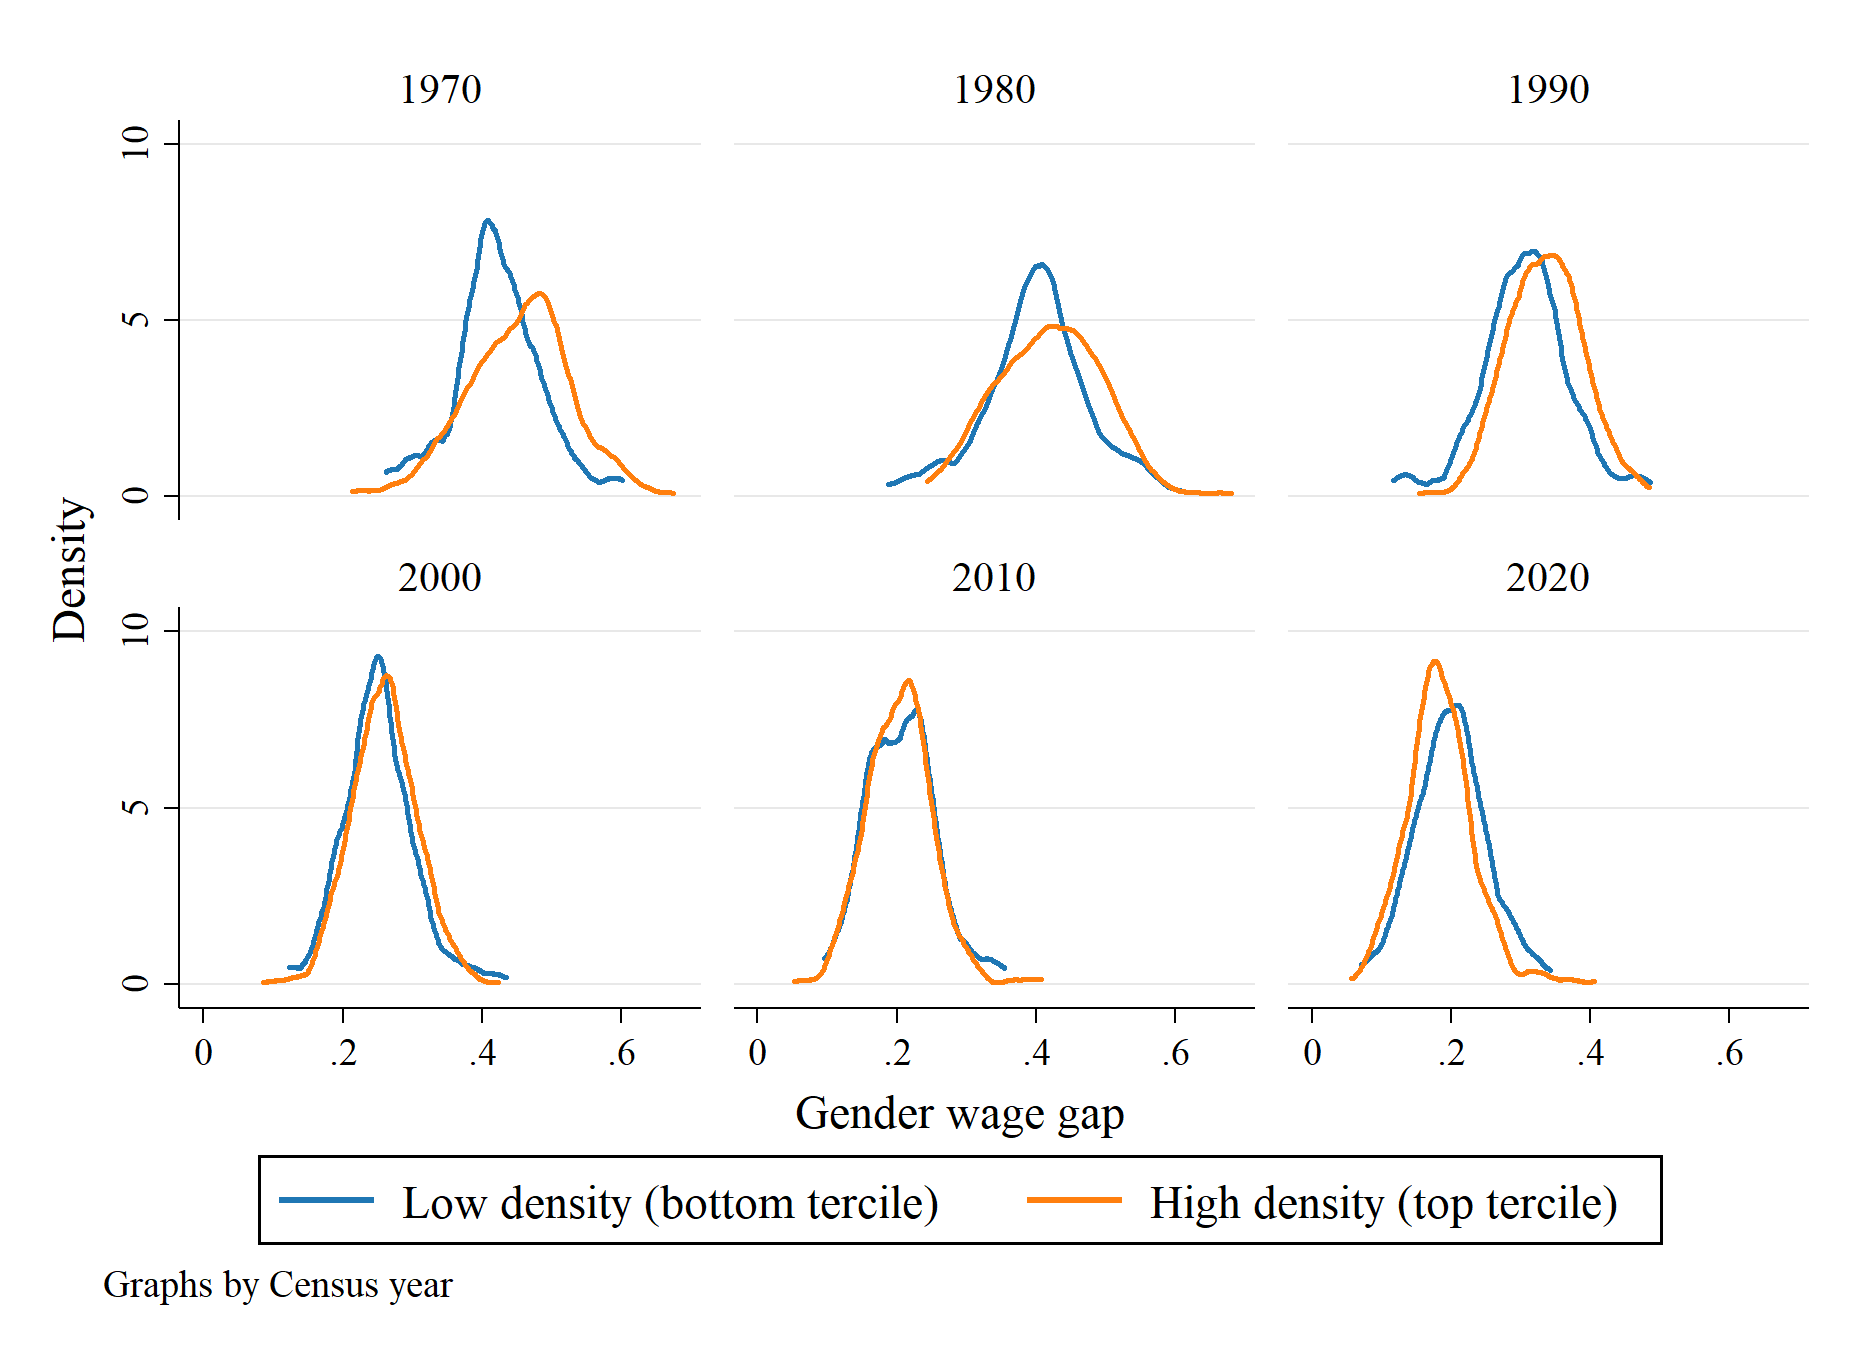
\includegraphics[width=.8\textwidth]{../2_analysis/output/figures/distribution_gap_movement_full_time}
\par \begin{minipage}[h]{\textwidth}{\scriptsize\textbf{Note:} figure restricts to CZ with more than 1 people per km$^2$. Figure generated on 28 Sep 2020 at 15:56:45. Figure generated using the dofile code\_files/kernel\_density\_movement.do.}\end{minipage}
\end{figure}

	\beamerbutton{\hyperlink{slide:baseline}{Return}}
\end{frame}